%
\documentclass{article} % For LaTeX2e
\usepackage{iclr2016_conference,times}
\usepackage{url}
\usepackage{latexsym}

\usepackage{times}
\usepackage{caption}
\usepackage[scientific-notation=true]{siunitx}
\usepackage{amsmath}
\usepackage{amsthm}
\usepackage{amssymb}
\usepackage{graphicx}
\usepackage{xspace}
\usepackage{tabularx}
\usepackage{multicol}
\usepackage{multirow}
%\usepackage{hyperref}
\usepackage{url}
%\usepackage{natbib}
\usepackage{wrapfig}
\usepackage{comment}
\usepackage{listings}
\usepackage{color}
\usepackage[utf8]{inputenc}
\usepackage{fancyvrb}
\usepackage{booktabs}
\usepackage{color}
\usepackage[normalem]{ulem}

\newcommand{\obs}{\text{obs}}
\newcommand{\mis}{\text{mis}}

\newcommand{\qt}[1]{\left<#1\right>}
\newcommand{\ql}[1]{\left[#1\right]}
\newcommand{\hess}{\mathbf{H}}
\newcommand{\jacob}{\mathbf{J}}
\newcommand{\hl}{HL}
\newcommand{\cost}{\mathcal{L}}
\newcommand{\lout}{\mathbf{r}}
\newcommand{\louti}{r}
\newcommand{\outi}{y}
\newcommand{\out}{\mathbf{y}}
\newcommand{\gauss}{\mathbf{G_N}}
\newcommand{\eye}{\mathbf{I}}
\newcommand{\softmax}{\phi}
\newcommand{\targ}{\mathbf{t}}
\newcommand{\metric}{\mathbf{G}}
\newcommand{\sample}{\mathbf{z}}
\newcommand{\f}{\text{f}}
%\newcommand{\log}{\text{log}}

\newcommand{\bmx}[0]{\begin{bmatrix}}
\newcommand{\emx}[0]{\end{bmatrix}}
\newcommand{\qexp}[1]{\left<#1\right>}
\newcommand{\vect}[1]{\mathbf{#1}}
\newcommand{\vects}[1]{\boldsymbol{#1}}
\newcommand{\matr}[1]{\mathbf{#1}}
\newcommand{\var}[0]{\operatorname{Var}}
\newcommand{\std}[0]{\operatorname{std}}
\newcommand{\cov}[0]{\operatorname{Cov}}
\newcommand{\diag}[0]{\operatorname{diag}}
\newcommand{\matrs}[1]{\boldsymbol{#1}}
\newcommand{\va}[0]{\vect{a}}
\newcommand{\vb}[0]{\vect{b}}
\newcommand{\vc}[0]{\vect{c}}
\newcommand{\ve}[0]{\vect{e}}

\newcommand{\vh}[0]{\vect{h}}
\newcommand{\vv}[0]{\vect{v}}
\newcommand{\vx}[0]{\vect{x}}
\newcommand{\vz}[0]{\vect{z}}
\newcommand{\vw}[0]{\vect{w}}
\newcommand{\vs}[0]{\vect{s}}
\newcommand{\vf}[0]{\vect{f}}
\newcommand{\vi}[0]{\vect{i}}
\newcommand{\vo}[0]{\vect{o}}
\newcommand{\vy}[0]{\vect{y}}
\newcommand{\vg}[0]{\vect{g}}
\newcommand{\vm}[0]{\vect{m}}
\newcommand{\vu}[0]{\vect{u}}
\newcommand{\vL}[0]{\vect{L}}
\newcommand{\vr}[0]{\vect{r}}
\newcommand{\vp}[0]{\vect{p}}
\newcommand{\mW}[0]{\matr{W}}
\newcommand{\mP}[0]{\matr{P}}

\newcommand{\mE}[0]{\matr{E}}
\newcommand{\mG}[0]{\matr{G}}
\newcommand{\mX}[0]{\matr{X}}
\newcommand{\mQ}[0]{\matr{Q}}
\newcommand{\mU}[0]{\matr{U}}
\newcommand{\mF}[0]{\matr{F}}
\newcommand{\mV}[0]{\matr{V}}
\newcommand{\mA}{\matr{A}}
\newcommand{\mC}{\matr{C}}
\newcommand{\mD}{\matr{D}}
\newcommand{\mS}{\matr{S}}
\newcommand{\mI}{\matr{I}}
\newcommand{\td}[0]{\text{d}}
\newcommand{\TT}[0]{\vects{\theta}}
\newcommand{\PP}[0]{\vects{\phi}}
\newcommand{\vsig}[0]{\vects{\sigma}}
\newcommand{\valpha}[0]{\vects{\alpha}}
\newcommand{\vmu}[0]{\vects{\mu}}
\newcommand{\vzero}[0]{\vect{0}}
\newcommand{\tf}[0]{\text{m}}
\newcommand{\tdf}[0]{\text{dm}}
\newcommand{\grad}[0]{\nabla}
\newcommand{\alert}[1]{\textcolor{red}{#1}}
\newcommand{\N}[0]{\mathcal{N}}
\newcommand{\LL}[0]{\mathcal{L}}
\newcommand{\HH}[0]{\mathcal{H}}
\newcommand{\NN}[0]{\mathcal{N}}
\newcommand{\RR}[0]{\mathbb{R}}
\newcommand{\II}[0]{\mathbb{I}}
\newcommand{\Scal}[0]{\mathcal{S}}
\newcommand{\sigmoid}{\text{sigmoid}}
\newcommand{\Bernoulli}{\text{Bernoulli}}
\newcommand{\E}[0]{\mathbb{E}}
\newcommand{\enabla}[0]{\ensuremath{%
    \overset{\raisebox{-0.3ex}[0.5ex][0ex]{%
    \ensuremath{\scriptscriptstyle e}}}{\nabla}}}
\newcommand{\enhnabla}[0]{\nabla_{\hspace{-0.5mm}e}\,}

\renewcommand*{\thefootnote}{\fnsymbol{footnote}}

\newcommand{\todo}[1]{{\Large\textcolor{red}{#1}}}
\newcommand{\done}[1]{{\Large\textcolor{green}{#1}}}
\newcommand{\dd}[1]{\ensuremath{\mbox{d}#1}}

\DeclareMathOperator*{\argmax}{\arg \max}
\DeclareMathOperator*{\argmin}{\arg \min}
\newcommand{\newln}{\\&\quad\quad{}}

\newcommand{\Ax}{\mathcal{A}_x}
\newcommand{\Ay}{\mathcal{A}_y}
\newcommand{\ola}{\overleftarrow}
\newcommand{\ora}{\overrightarrow}
\newcommand{\ov}{\overline}
\newcommand{\ts}{\rule{0pt}{2.6ex}}       % Top strut
\newcommand{\ms}{\rule{0pt}{0ex}}         % Middle strut
\newcommand{\bs}{\rule[-1.2ex]{0pt}{0pt}} % Bottom strut
\newcommand{\specialcell}[2][c]{%
  \begin{tabular}[#1]{@{}c@{}}#2\end{tabular}}

%\newcommand\codeHighlight[1]{\textcolor[rgb]{1,0,0}{\textbf{#1}}}
\newcommand\codeHighlight[1]{\textcolor[rgb]{1,0,0}{#1}}

%\title{Larger-Context Language Modelling \\ with Recurrent Neural Network}
\title{Iterative Refinement of \\ Approximate Posterior for \\ Training Directed Belief Networks}

\author{R Devon Hjelm \\
Mind Research Network \\ \& the University of New Mexico \\
\texttt{\small dhjelm@mrn.org} 
\And
Kyunghyun Cho \\
Courant Institute \\ \& Center for Data Science \\
New York University \\
\texttt{\small kyunghyun.cho@nyu.edu}
\And
Junyoung Chung \\
University of Montreal \\
\texttt{\small junyoung.chung@umontreal.ca}
\And
Russ Salakhutdinov \\
University of Toronto \\
\texttt{\small rsalakhu@cs.toronto.edu}
\And
Vince Calhoun \\
Mind Research Network \\ \& the University of New Mexico \\
\texttt{\small vcalhoun@mrn.org}
\And
Yoshua Bengio \\
University of Montreal \\
\texttt{\small yoshua.bengio@umontreal.ca}
\And
Nebojsa Jojic \\
Microsoft Research \\
\texttt{\small jojic@microsoft.com}
}

% The \author macro works with any number of authors. There are two commands
% used to separate the names and addresses of multiple authors: \And and \AND.
%
% Using \And between authors leaves it to \LaTeX{} to determine where to break
% the lines. Using \AND forces a linebreak at that point. So, if \LaTeX{}
% puts 3 of 4 authors names on the first line, and the last on the second
% line, try using \AND instead of \And before the third author name.

\newcommand{\fix}{\marginpar{FIX}}
\newcommand{\new}{\marginpar{NEW}}

%\iclrfinalcopy % Uncomment for camera-ready version

\begin{document}

\maketitle

\begin{abstract}
    Deep directed graphical models, while a potentially powerful
    class of generative representations, are challenging to train due to difficult inference. Recent advances in variational inference that make use
    of an inference or \emph{recognition network} have advanced well beyond
    traditional variational inference and Markov chain Monte Carlo methods. While these techniques
    offer higher flexibility as well as simpler and faster inference, they are
    still limited by the choice of approximate posterior and require variance
    reduction techniques. Less focus has been given to improving or \emph{refining} the
    approximate posterior beyond what is provided by variational inference. We
    show that iterative refinement of the approximate posterior can provide
    notable gains in maximizing the lower bound of the log likelihood, either
    by applying gradient descent or by using adaptive importance sampling
    during the E-step of a variational expectation-maximization algorithm. We show our approach
    competes with state of the art in both continuous and binary latent
    variables.
    \end{abstract}

\section{Introduction}

Deep generative models offer the capacity for rich representations of complex
data as they can capture multimodal properties of the distribution of
interest and generalize better than models based purely on deterministic processes. Deep directed
graphical models in particular have some advantage over their undirected
cousins such as deep Boltzmann machines \citep[DBMs,][]{salakhutdinov2009deep} as they do not suffer from
learning and evaluation difficulties arising from an intractable partition
function. Despite their representational power, directed graphical models are
often difficult to train, as the true posterior is generally intractable.

Methods for training variants of the Helmholtz machine
\citep{dayan1995helmholtz}, such as wake-sleep \citep{hinton1995wake,
bornschein2014reweighted} and neural variational inference and learning
\citep[NVIL,][]{mnih2014neural}, and methods for training variational
autoencoders~ \citep[VAE,][]{kingma2013auto} have supplanted more traditional
Markov chain Monte Carlo (MCMC) \citep{neal1992connectionist} or variational
inference based methods such as mean field coordinate ascent inference
\citep{saul1996mean} in training deep generative models. The gains offered by
these methods are due to parameterizing the approximate posterior with a
\emph{recognition network} on top of clever learning algorithms. As opposed to
traditional methods, this general approach provides a fast and effective means
of performing inference and learning which scales well to large datasets.

While advances have been clear, these methods are still limited by the choice
of approximate posterior, which translates to a looseness in the lower bound.
Some recent work has begun to address this limitation by either relaxing the
factorial assumption \citep{burda2015importance} on the approximate posterior or
through the introduction of auxiliary inference networks
\citep{rezende2015variational}.

There has been recent focus on
refining the variational posterior by applying gradient descent to variational
inference \citep{hoffman2013stochastic} or by applying additional MCMC
transitions \citep{salimans2014markov}. We demonstrate two different methods to
refine the approximate posterior from the recognition network during the E-step
of an expectation-maximization~\citep[EM,][]{dempster1977maximum, neal1998view})
algorithm to improve the variational lower bound. 
We first show that, given lower bound optimization can be
reinterpreted in terms of a deterministic function with auxiliary noise, we can use simple gradient descent
to refine the approximate posterior during inference. Next, we show that with
binary latent variables, adaptive importance sampling
\citep[AdIS][]{karamchandani1989adaptive} can be used instead of gradient descent.

\section{Directed Belief Networks and Variational Inference}

The term \emph{belief network} describes a class of generative models of which
the observed distribution is conditioned on a set of stochastic latent causes:
$p(x) = \sum_h p(x|h) p(h)$, though in general this term is used to include
models where the observed variables are not conditionally independent on the
latent variables, $h$. 

In this work, we will use the name \emph{directed belief network} to restrict
ourselves to a generative directed graphical model such that the likelihood
function factorizes into a hierarchy of conditional densities: $p(x | h) =
p(h_n) p(x|h_1) \prod_{l=1}^n p(h_{l}|h_{l+1})$, where each layer $l$ is
conditionally independent on the layer above with density $p(h_{l}|h_{l + 1})$
and $p(h_n)$ is a prior distribution of the top layer. Examples include sigmoid
belief networks \citep[SBN,][]{neal1992connectionist} and deep belief networks
\citep[DBN,][]{hinton2006fast}.

Directed belief networks can be trained by maximizing log-likelihood (MLE), but
this is difficult due to the necessary marginalization over the latent density.
If we had the posterior $p(h|x) = p(x, h) / p(x)$, then learning would be straightforward,
but in general this is not possible and requires more advanced
techniques. 

\section{Variational Inference and Learning of \\ Directed Belief Networks}

\subsection{Variational Lowerbound of Directed Belief Network}

Even with a reasonably complex likelihood function, MLE is not tractable in
directed belief networks due to the intractable posterior inference.  One
solution is to use MCMC sampling to iteratively approximate the posterior
distribution over the latent variables, which is exact given an unbound number
of steps under certain conditions. This typically suffers from high variance in its
gradient estimates.

Another popular method, variational inference introduces an approximate
posterior $q_{\TT}(h|x)$:
\begin{align}
    \label{eq:approx_logp}
    \log p(x) =& \log \sum_{h} p(x, h) 
    = \log \sum_h q(h|x) \frac{p(x, h)}{q(h|x)} \nonumber \\
    \geq& \sum_h q(h|x) \log \frac{p(x, h)}{q(h|x)} 
    = \sum_h q(h|x) \log p(x,h) + \HH(q) = \LL,
\end{align}
with variational parameters $\TT$, where $\HH(q)$ is the entropy of the
approximate posterior $q$. 

This introduces \emph{lower bound}, $\LL$, of the exact likelihood. Variational
inference rephrases learning as choosing the variational parameters $\TT$ to
maximize this bound, rather than choosing the latent variables directly. The
bound is tight (i.e., $\LL = \log p(x)$) when the KL divergence between the
approximate and true posterior is $0$ (i.e., $D_{KL}(q_{\TT}(h|x)||p(h|x)) =
0$); or equivalently when the approximate matches the true posterior.
Optimization then is dependent on the choice of a parametric form for the
posterior that can best approximate the exact posterior, and models generally
vary in choice of parameterization followed by a learning algorithm which
efficiently maximizes its lower bound.

\subsection{Training a Directed Belief Network}

If we have a method for finding an approximate posterior, then learning follows an
EM algorithm.  In the E-step, the variational parameters of the approximate posterior, $\TT$,
are chosen/updated such that the KL-divergence between the approximate posterior and
true posterior is minimized. In the maximization (M) step, the model parameters
$\PP$ are chosen/updated to maximize the likelihood function.

In general, the gradient w.r.t. the model parameters of the lower bound can be
estimated using the following Monte Carlo approximation:
\begin{align} \label{eq:grad}
\nabla_{\PP} \LL \approx \frac{1}{N} \sum_n \nabla_{\PP} \log p_{\PP}(x, h^{(n)}),
\end{align}
where $h^{(n)} \sim q(h|x)$.

\subsection{Recognition Network}

Recently, it has been found that the approximate posterior inference can be done
quickly by using a feed forward, often deep, \emph{recognition network} composed
of \emph{global} variational parameters to predict the local variational
parameters from the data \citep[see,
e.g.,][]{kingma2013auto,mnih2014neural,rezende2014stochastic}. However, these
approaches often require additional tricks to train, as the gradient of the
lower bound w.r.t. the global variational parameters is difficult to compute,
and most of the off-the-shelf approximations, such as Monte Carlo approximation,
have high variance. 

Variational autoencoders \citep[VAE,][]{kingma2013auto} make use of a clever
parameterization trick so that the lower bound can be rephrased as a
deterministic function with some auxiliary noise. The wake-sleep algorithm uses
samples from the joint density $p(x, h)$ to optimize the variational parameters,
effectively making the algorithm an optimization over two cost functions
\citep{hinton1995wake}. NVIL
uses REINFORCE \citep{williams1992simple} along with a baseline predicted from a deep neural network to
make lower variance MCMC estimates of the gradient.

It can be argued that better estimates can be made by simply having a better
posterior. Some work has proposed to use gradient descent
\citep{hoffman2013stochastic}, auxiliary networks
\citep{rezende2015variational}, or MCMC transitions \citep{salimans2014markov}
to refine inference with various posterior parameterizations. 

In general, we want an iterative refinement procedure, defining a transition
operator $T$ that arrives at a better posterior, $\tilde{q}$, when applied
iteratively to approximate posterior, $q$. 
%We then adjust our global variational
%parameters by minimizing the KL divergence, $D_{KL}(\tilde{q}||p)$.

\section{Iterative Refinement for Variational Inference (IRVI)}

\subsection{Iterative Refinement of Approximate Posterior}
We restrict ourselves to the case where the prior and approximate posterior are
factorial, that is: $p(h) = \prod_i p(h_i)$ and $\tilde{q}(h|x; \TT) = \prod_i
\tilde{q}(h_i|x; \TT)$, respectively. The method relies on an initial set of \emph{local} variational parameters, $\TT^l$, optionally a function of the data
such as ones given from a recognition network. Given a lower bound $\LL(\theta^l)$, we achieve a better posterior, maximizing $\LL$, by taking iterative steps 
in $\TT^l$, using a series of transition operators $T(\TT^l_t, \TT^l_{t-1}; \LL)$. 
The only criteria on the transition operators, $T$, is that they should be parameterized by and maximize $\LL$.

After we find $\tilde{q}$, parameterized by an optimal set of variational parameters $\TT^{l\star}$, we maximize the lower bound w.r.t. the model
parameters using stochastic gradient descent, using samples from the refined
approximate posterior. Learning for the model parameters follows equation \ref{eq:grad}, and the loss w.r.t. the global variational parameters becomes
$D_{KL}(\tilde{q}(\theta^l)||q_{\TT})$.

\subsubsection{Gradient Descent Iterative Refinement (GDIR)}
If we can rephrase the lower bound as a deterministic function $g(\TT^l; \epsilon)$ of the local
variational parameters and some optional auxiliary noise variables, $\epsilon$,
then we are guaranteed to improve the local variational parameters by applying iterative steps
of gradient ascent:

\begin{align}
\grad_{\TT^l} \LL &\approx \grad_{\TT^l} g(\TT^l, \epsilon) \nonumber \\
\TT^l_t &= \TT^l_{t-1} + \gamma \grad_{\TT^l} g(\TT^l, \epsilon)
\end{align}
where $\gamma$ is the "inference rate" and $\TT^l_0$ are the initial local
parameters found through the initial variational inference. The success of this
approach will depend on the choice of approximation, which we will show.

\paragraph{Gaussian Latent Variables}

Let us assume that our approximate posterior and prior distributions are
parameterized by multivariate normal distributions with diagonal covariance. In
order to pass the gradient of the approximate log conditional to the variational
parameters, we can use the re-parameterize our approximate posterior as in VAE:
\begin{align}
h(\TT^l) &= \mu + \epsilon \odot \sigma \nonumber \\
\epsilon &\sim \NN(0, 1),
\end{align}
where $(\mu, \sigma) = \TT^l$ are the mean and variance parameters for the
posterior density and our auxiliary noise variables, $\epsilon$, are sampled
from a unit-variance, zero-mean normal distribution.

The gradient of the lower bound w.r.t. the local variational parameters can be
approximated easily by Monte Carlo method:
\begin{align}
\grad_{\TT^l} g(\TT^l, \epsilon) = \frac{1}{N} \grad_{\TT^l} \bigg(\sum_n \log p(x, h(\TT^l)^{(n)}) - \log \tilde{q}(h(\TT^l)^{(n)})\bigg).
\end{align}

\paragraph{Bernoulli Latent Variables}
Unfortunately, a suitable re-parameterization as above is not available to us
with binary latent variables. In order to use gradient descent to back-propagate
the gradients of the lower bound, we need to make a stronger approximation. 

There has been some recent work into passing gradients through binary latent
variables \citep{bengio2013estimating}. Instead of approximating the partial
derivatives w.r.t. the latent variables in back-propagation, we instead push the
centers of the Bernoulli distribution, avoiding sampling overall. Our lower
bound becomes:
\begin{align}
     \LL \approx g(\TT^l) = \log p(x | \mu) + \qexp{\log p(h)}_{\tilde{q}} +
     \HH(\tilde{q}),
\end{align}
where $\log p(x | \mu)$ is the log-output of the generation network using the
variational parameters $\mu = \sigmoid(z)$ as input. However, this approximation
is likely highly biased, and becomes worse as $\mu$ moves away from $(0, 1)$, so
we would expect this approximation to be best when $\HH(\tilde{q})$ is small.

\subsubsection{Adaptive Importance Sampling Iterative Refinement (AIR)}
As an alternative to and to address the issues with the binary latent variable approximation above, we use \emph{adaptive importance sampling} \citep[AdIS,][]{karamchandani1989adaptive} to iteratively refine the Bernoulli centers at each inference step:

\begin{align}
    h^{(n)} &\sim \Bernoulli(\mu_t) \nonumber \\
w^{(n)} &= p(x, h^{(n)}) / q(h^{(n)} | x) \nonumber \\
\tilde{w}^{(n)} &= w^{(n)} / \sum_n w^{(n)} \nonumber \\
\mu_{t+1} &= \mu_t + \gamma \grad_{\TT^l} g(\TT^l) \nonumber\\
\grad_{\TT^l} \LL \approx \grad_{\TT^l} g(\TT^l) &= q_t - \mu_t  = \sum_n
    \tilde{w}^{(n)} h^{(n)} - \mu_t,
\end{align}

where $\gamma$ is the learning rate and $(1 - \gamma)$ can be though of as the adaptive "damping" rate. Adaptive importance sampling "recenters" the proposed distribution using a weighted average of samples from said distribution, weighting by the importance weights. This will clearly lead to a biased estimate of the lower bound when with a finite number of samples from $\tilde{q}$. However, we will show that it works very well in practice. This approach is simpler for binary variables, as the distribution is parameterized Bernoulli centers, than for Gaussian variables which have both mean and covariance. Though it may be applicable, AIR with Gaussian variables is not explored here.

\section{Related Works}
IRVI combines elements found in variational inference and MCMC methods. In
spirit, it is closest to the refinement procedure of hybrid MCMC for variational
inference \citep[HVI,][]{salimans2014markov}, and in some senses HVI can be thought as a type of iterative refinement. However, the MCMC transitions in GDIR and AIR are substantially simpler than those used in HVI. In addition, HVI
requires same re-parameterization trick as in VAE, as is used in GDIR, limiting it's application to continuous latent variables.

Our work also shares similarities with stochastic variational inference
\citep{hoffman2013stochastic} also uses gradient descent to improve on the
variational inference algorithm. However, the exact parameterization of the
posterior is very limited and the method cannot be used with complex approximate
posteriors. 

Normalizing flows for VAE \citep[NF]{rezende2015variational} make use of auxiliary
networks to improve the approximate posterior. In doing so, they are able to
escape the factorial condition that GDIR and AdISIR have. However, NF requires
additional parameters to improve the posterior as well as a complex learning
algorithm, as it requires the choice of a parametric and invertible transformation.

Importance sampling has shown to be successful in achieving better gradient
estimates, such as in re-weighted wake-sleep \citep[RWS,
][]{bornschein2014reweighted}, importance-weighted autoencoders
\citep[IWAE,][]{burda2015importance}, and work on stochastic feed-forward
networks \citep[SFFN, ][]{tang2013learning}. Iterative refinement, however, takes a distinct approach, as it uses
importance sampling instead to achieve a better posterior through refinement.

Finally, IRVI is not entirely orthogonal to many variational inference methods, and could be combined to enhance results, particularly with variational inference methods that follow an EM training procedure.

\section{Experiments}

\subsection{Settings}

We test GDIR and AIR on MNIST, using the benchmark binarized dataset found in
\citep{salakhutdinov2008quantitative}, with a standard train, validation, and
test split of $50$k, $10$k, and $10$k samples. We centered the entire MNIST dataset by subtracting the mean digit over the corresponding dataset (train, valid, and test). Unfortunately, recent papers on
VAE \citep{mnih2014neural, salimans2014markov} have used different, non-standard
splits, or actively sample from continuous MNIST \citep{burda2015importance},
making it difficult to compete. We however make sure that our results are from
the most conservative setting (having the least amount of training examples and
binarizing only once),
thereby making any comparison as meaningful as possible.

All models used a recognition network for comparison to similar models, with
the number of parameters and deterministic layers (if present) matching the
generation network. Models were trained using the the RMSprop algorithm
\citep{Hinton-Coursera2012}, with a batch size of $100$, with early stopping by
recording best validation lowerbound. All models were tested using $1000$ posterior samples
to estimate the lower bounds and log likelihoods.

\subsection{Continuous Variables}
For continuous latent variables, we used the same network structure as in
\citep{kingma2013auto, salimans2014markov}, with $200$ latent variables and a
generation and recognition network with $500$ intermediate deterministic
softplus ($\log (1 + \exp(x))$) units. We excluded the mean and variance parameters for the prior constant at zero mean and unit variance.
Each of our models were trained using using an initial learning
rate of \num{0.0001}, an inference rate of \num{0.003}, $20$ or $50$ samples
during inference using GDIR to refine output of the recognition network, and
$20$ or $50$ samples to approximate the lower bound during the M-step; with all
hyper-parameters chosen from validation runs. In order to demonstrate the effect
of inference steps on learning, we varied the number of inference steps from
$1$, $5$, $10$, $20$, and $50$.

All models were trained for $1000$ epochs with the initial learning rate,
followed by $100$ epochs at a learning rate of \num{0.00001}, and finished with
$100$ epochs of \num{0.000001}. We also used $L2$ weight decay with a decay
coefficient of \num{0.0002}. During test, all models were evaluated using $50$
inference steps during the E-step when refining the approximate posterior.

Our test results with continuous latent variables (GDIR) are presented in Table
\ref{table:continuous} with the number of posterior samples, $K$, and inference
steps, $n$, specified as $GDIR_{K, n}$, with $K=20$ and $n=20$ chosen from
validation. For comparison are
(approximate) VAE results \alert{(They just have plots, no numbers)} from
\citep{kingma2013auto}, deep latent gaussian models with normalizing flow
\citep[DLGM+NF,][]{rezende2015variational}, HVI with the number of leapfrog steps
specified, and IWAE. Included in Table \ref{table:cont_step} is
the effect of inference steps during training on the lower bound and log
likelihood.

GDIR shows notable improvement over VAE, while showing comparable performance to
Hamiltonian MCMC with 5 leapfrog steps, despite conservative training.
Performance falls short of HVI with $10$ leapfrog steps, IWAE, and DLGM+NF (diagonal covariance),
though differences in model and training specification make a direct comparison difficult.

We observe that the number of inference steps during training improves lower
bound and log likelihood estimates. In addition, the bound becomes tighter both
as the number of inference during training and during evaluation (Figure \ref{fig:continuous}).

\begin{minipage}{\textwidth}
    \begin{minipage}[l]{0.5\textwidth}
        \begin{tabular}{ | m{8em} | m{1.4cm} | m{1.4cm} | } 
            \hline
            Model & $\ge$ -log(x) & $\approx$ -log(x) \\ 
            \hline
            \hline
            VAE \textasteriskcentered & 99 &  \\ 
            \hline
            \hline
            $GDIR_{20, 20}$ & 91.89 & 89.51 \\ 
            $GRID_{50, 20}$ & 91.80 & 89.42 \\
            \hline
            \hline
            $HVI_5$\textdagger &  90.86 & 87.16 \\ 
            $HVI_{10}$\textdagger & 87.60 & 85.56 \\ 
            \hline
            DLGM+NF & 89.9 &\\
            \hline
            IWAE ($K=50$)\textdaggerdbl & & 84.78 \\ 
            \hline
        \end{tabular}
    \captionof{table}{Lower bounds and NLL for various continuous latent variable models and training algorithms. \textasteriskcentered{Approximate value from \cite{kingma2013auto}.} \textdagger{Using the Larochelle dataset and validation dataset during training}. \textdaggerdbl{Sampling from continuous MNIST and using an additional linear layer and parameters to model the mean.}}
    \label{table:continuous}
    \end{minipage}
    \hspace{0.05\textwidth}
    \begin{minipage}[r]{0.43\textwidth}
        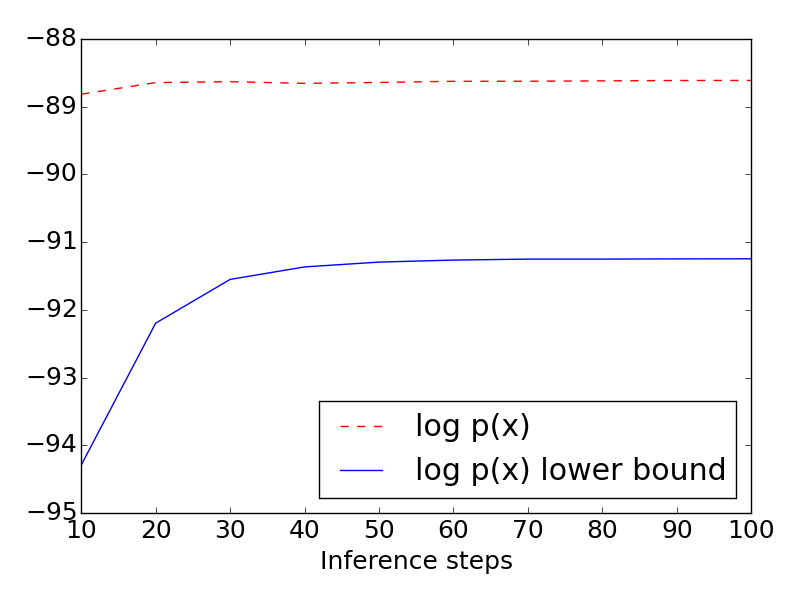
\includegraphics[scale=0.3]{figures/continuous_eval}
        \captionof{figure}{Log likelihood and lower bound for a single continuous latent variable
        model with varying number of inference steps during test over a subset of $500$
        samples from the test data.}
        \label{fig:continuous}
        \end{minipage}
\end{minipage}

\begin{table}
\begin{tabular}{ | m{1.4cm} | m{1cm} | m{1cm} | m{1cm} | m{1cm} | m{1cm} |}
\hline
n & 1 & 5 & 10 & 20 & 50 \\
\hline
$\ge$ -log(x) & 96.24 & 93.72 & 93.36 & 91.89 & \\
\hline
$\approx$ -log(x) & 95.24 & 91.59 & 90.85 & 89.51 & \\
\hline
\end{tabular}
\caption{Results for models trained with GDIR with number of steps, $n$, during training. Each model was evaluated using $50$ steps during inference.}
\label{table:cont_step}
\end{table}

\subsection{Bernoulli Variables}
For binary latent variables, we used two different parameterizations in order compare to shallow and 2-layer wake-sleep and
NVIL using both GDIR and AIR. For comparison to wake-sleep, we used a shallow
feed-forward network with $200$ output neurons, $z$, for the local variational parameters as $\TT^l = \mu = \sigmoid(z)$, with no additional deterministic units, for both the recognition and generation nets.
As NVIL uses an additional feed forward network for baseline prediction, we added
an intermediate deterministic layer with $240$ softplus units in both the recognition and generation
networks to roughly match the total number of parameters between each model. Models
were trained using an initial learning rate of \num{0.001} and $20$ samples
during inference, and $20$ posterior samples were used to estimate the lower bound during the
M-step.

To demonstrate IRVI with multiple layers, we used an SBN with a generation network with a structure of 200-200 binary latent layers and a generation network with a matched parameterization. However, for our approximate posterior we treated the outputs of each layer as the factors of the complete approximate posterior, that is $q(h1, h2 | x) = q(h1|x) q(h2|x)$, where $q(h2|x)$ shares the lower-level parameters with those of $q(h1|x)$. This allows us to adapt the Bernoulli means of $h1$ and $h2$ simultaneously, without having to account for dependencies.

Single-layer GDIR and AIR models were trained with $1$, $5$, $10$, $20$, and $50$ inference steps, while the 2-layer SBN was trained only with $50$ inference steps. All
models were trained for $500$ epochs with the initial learning rate. For AIR, an
adaptive damping rate of $0.9$ was used, as lower damping rates proved unstable, though often gave competitive results.
During test, $100$ steps were used during inference for the single-layer SBN, while $300$ steps were used for the 2-layer SBN, and final models were selected
based on lower-bound validation performance.

\begin{minipage}{\textwidth}
    \begin{minipage}[l]{0.5\textwidth}

\begin{tabular}{ | m{8.7em} | m{1.4cm}| m{1.4cm} | } 
\hline
Model & $\ge$ -log(x) & $\approx$ -log(x) \\ 
\hline
\hline
Wake-sleep & 120.7 & 116.3 \\ 
WS (200-200) & 109.4 & 106.9 \\
RWS & & 103.1 \\
RWS (200-200) & & 93.4 \\
\hline
NVIL & 113.1 &  \\
NVIL (200-200) & 99.8 & \\ 
\hline
$AIR_{50}$ & 103.98 & 101.67 \\
$AIR_{20}$ (240 det sp) & 96.64 & 94.86 \\
$AIR_{50}$ (200-200) & 97.15 & 94.61 \\
\hline
$GDIR_{20}$ & 129.94 & 113.6 \\
$GDIR_{20}$ (240 det sp) & 118.28  & 104.22 \\
\hline
\end{tabular}
\captionof{table}{Results for GDIR and AIR for a single-layer SBN with and without an intermediate softplus layer of $240$ units and a 2-layer SBN compared to similar models trained on the same MNIST dataset.}
\label{table:binary}

\end{minipage}
    \hspace{0.05\textwidth}
    \begin{minipage}[r]{0.43\textwidth}

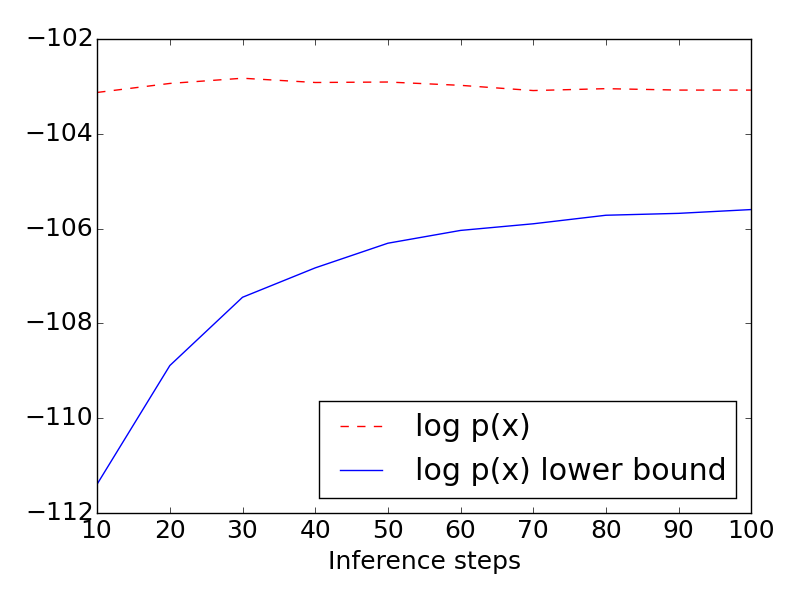
\includegraphics[scale=0.3]{figures/binary_eval}
\captionof{figure}{Log likelihood and lower bound for a single-layer binary latent variable
model with varying number of inference steps during test over a subset of $500$
samples from the test data.}
\label{fig:binary}
        \end{minipage}
\end{minipage}

\begin{table}
\begin{tabular}{ | m{1.4cm} | m{1cm} | m{1cm} | m{1cm} | m{1cm} | m{1cm} |}
\hline
n & 1 & 5 & 10 & 20 & 50 \\
\hline
$\ge$ -log(x) & 115.39 & 108.66 & 107.35 & 105.93 & 103.98 \\
\hline
$\approx$ -log(x) & 109.77 & 106.9 & 104.86 & 103.49 & 101.67 \\
\hline
\end{tabular}
\caption{Results for models without intermediate deterministic layer trained with AIR with number of steps, $n$, during training. Each model was evaluated using $100$ steps during inference.}
\label{table:binary_step}
\end{table}

The comparative results are compiled in table \ref{table:binary}. While GDIR does not perform nearly as well, AIR greatly outperforms NVIL, whether parameter-matched or not. In addition, AIR outperforms RWS in log likelihood estimates. As with continuous variables, we observe that higher number of inference steps during training (Table \ref{table:binary_step}) and during test (Figure \ref{fig:binary}) improves and tightens the lower bound.

\section{Conclusion}
We have introduced a unsophisticated method for improving variational inference using a transition operator that maximizes the lower bound which is flexible. We achieve comparable performance to methods for improving VAE, and achieve state-of-the-art results with a single layer SBN with RWS and comparable results on 2-layer SBN RWS.

\subsubsection*{Acknowledgments}
Work was partially funded by Microsoft Research and NIH\ grants R01EB005846 and P20GM103472 (to VDC).

\bibliography{ais_vae}
\bibliographystyle{iclr2016_conference}

\end{document}
